\documentclass[12pt, a4paper]{article}
\usepackage{subcaption}
\usepackage{ctex} % 支持中文处理
\usepackage{geometry} % 页面布局
\usepackage{graphicx} % 图片支持
\usepackage{hyperref} % 超链接支持
\usepackage{amsmath} % 数学公式
\usepackage{amsfonts}
\usepackage{amssymb}
\usepackage{amsthm}
\usepackage{bm}
\usepackage{color}
\usepackage{physics}
\newtheorem{lemma}{引理}
\newtheorem{theorem}{定理}
\geometry{left=2.5cm,right=2.5cm,top=2.5cm,bottom=2.5cm} % 设置页边距
\title{结果讨论}
\author{安庭毅\ 工学院 \ 2100011014}
\date{\today} % 使用今天的日期

\begin{document}

\maketitle % 显示标题
\section{流线及涡心绘制}
x和y方向均匀离散,网格点数N=401。由动力粘度$\nu = 0.001$设定雷诺数为1000。迭代计算至流场稳定后,通过寻找流函数局部极值的方式标记涡心,得到计算结果如下(区域记号采用Ghia论文中记法):
\begin{figure}[htbp]
    \centering
    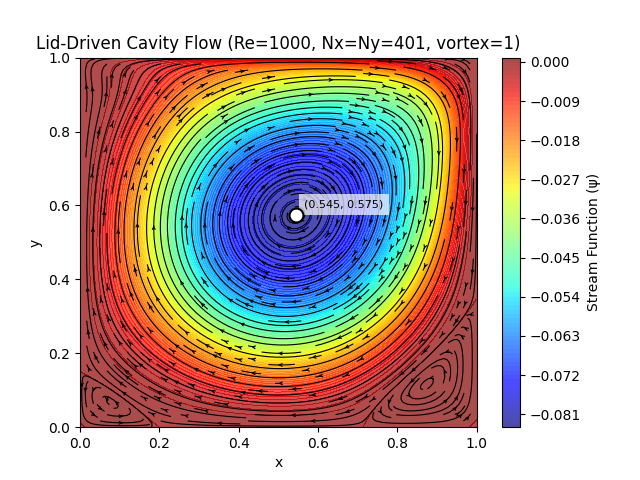
\includegraphics[width=\textwidth]{pictures/streamline_vortex_1.png}
    \caption{整体流线分布及主涡涡心位置}
\end{figure}

\begin{figure}[htbp]
    \centering
    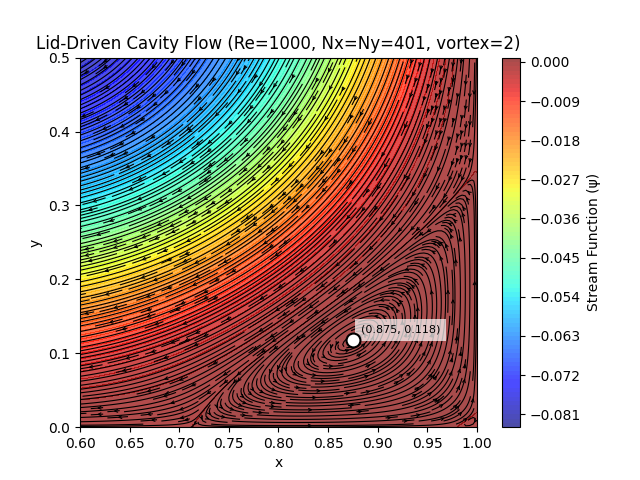
\includegraphics[width=\textwidth]{pictures/streamline_vortex_2.png}
    \caption{$H_{BR_{1}},V_{BR_{1}}$区域二次涡涡心位置}
\end{figure}

\begin{figure}[htbp]
    \centering
    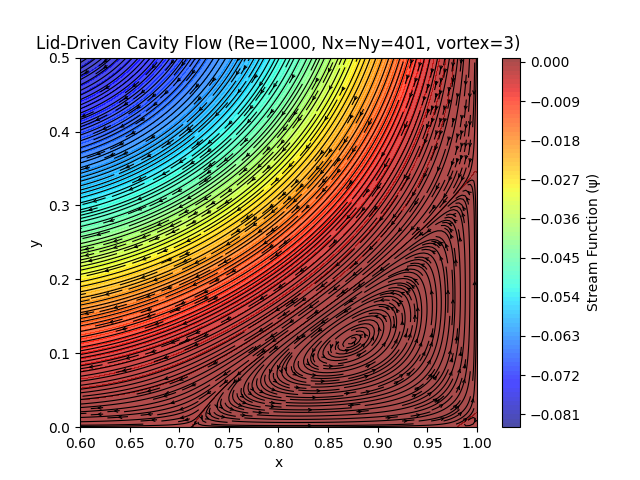
\includegraphics[width=\textwidth]{pictures/streamline_vortex_3.png}
    \caption{$H_{BL_{1}},V_{BL_{1}}$区域二次涡涡心位置}
\end{figure}

\begin{figure}[htbp]
    \centering
    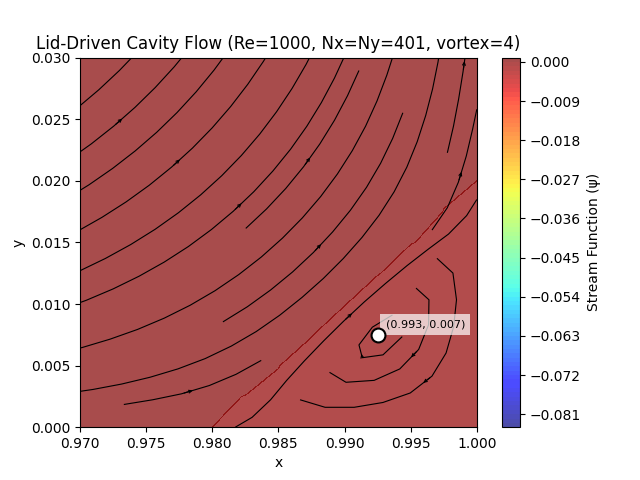
\includegraphics[width=\textwidth]{pictures/streamline_vortex_4.png}
    \caption{$H_{BR_{3}},V_{BR_{3}}$区域三次涡涡心位置}
\end{figure}

\begin{figure}[htbp]
    \centering
    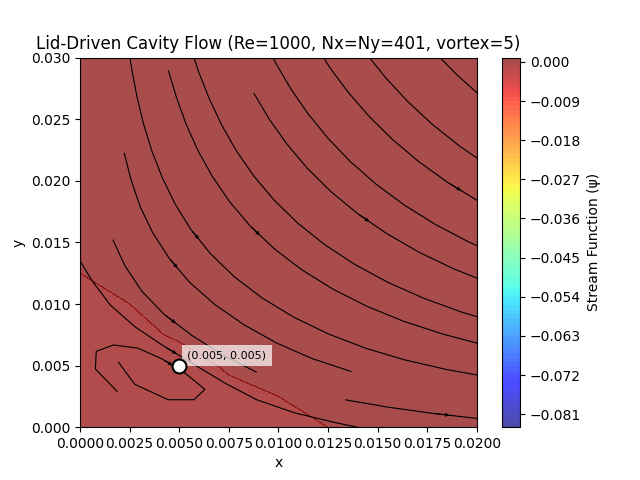
\includegraphics[width=\textwidth]{pictures/streamline_vortex_5.png}
    \caption{$H_{BL_{2}},V_{BL_{2}}$区域三次涡涡心位置(由于网格数量限制,误差较大)}
\end{figure}

以上流线与涡心位置与Ghia论文中Re=1000时的计算结果图样比较,吻合度较高,说明其正确性。

\section{垂直中线与水平中线的速度分布}
垂直中线的横向速度分布与水平中线的纵向速度分布如下所示:

\begin{figure}[htbp]
    \centering
    \begin{subfigure}[b]{0.48\textwidth}
        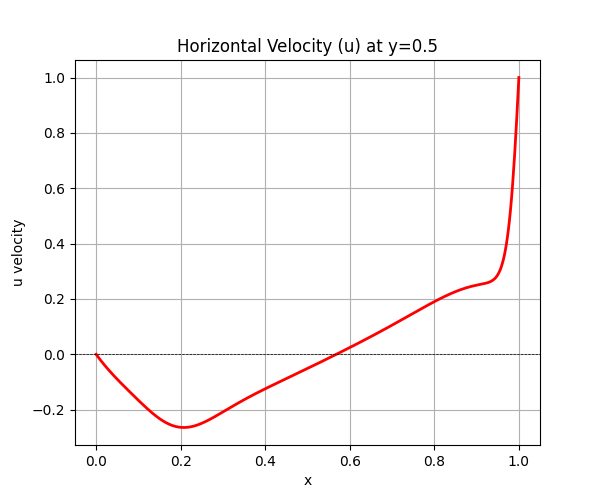
\includegraphics[width=\textwidth]{pictures/u_at_y_m.png}
        \caption{垂直中线的横向速度分布}
    \end{subfigure}
    \hfill
    \begin{subfigure}[b]{0.48\textwidth}
        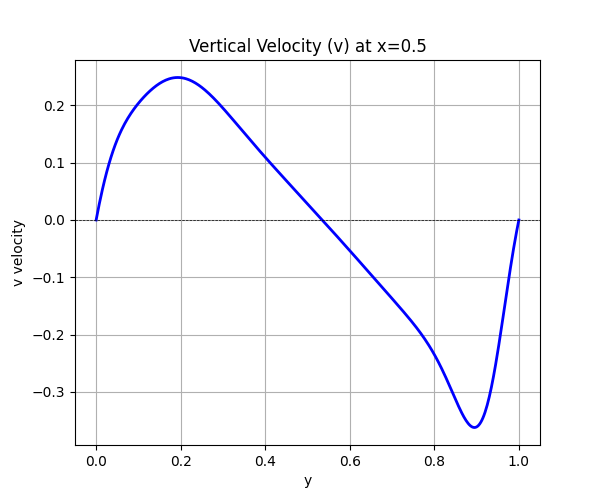
\includegraphics[width=\textwidth]{pictures/v_at_x_m.png}
        \caption{水平中线的纵向速度分布}
        \label{fig:sub2}
    \end{subfigure}
\end{figure}

以上结果与Ghia论文中图2a相比较类似。
\section*{附1:AI工具使用说明表}
使用的AI工具:deepseek和GPT-4o

AI生成代码行数及功能:plot.py中16-71行由AI生成(有自主修改),均为画图功能

核心代码自主编写比例:66\%

\section*{附2:git版本控制记录}
\begin{figure}[htbp]
    \centering
    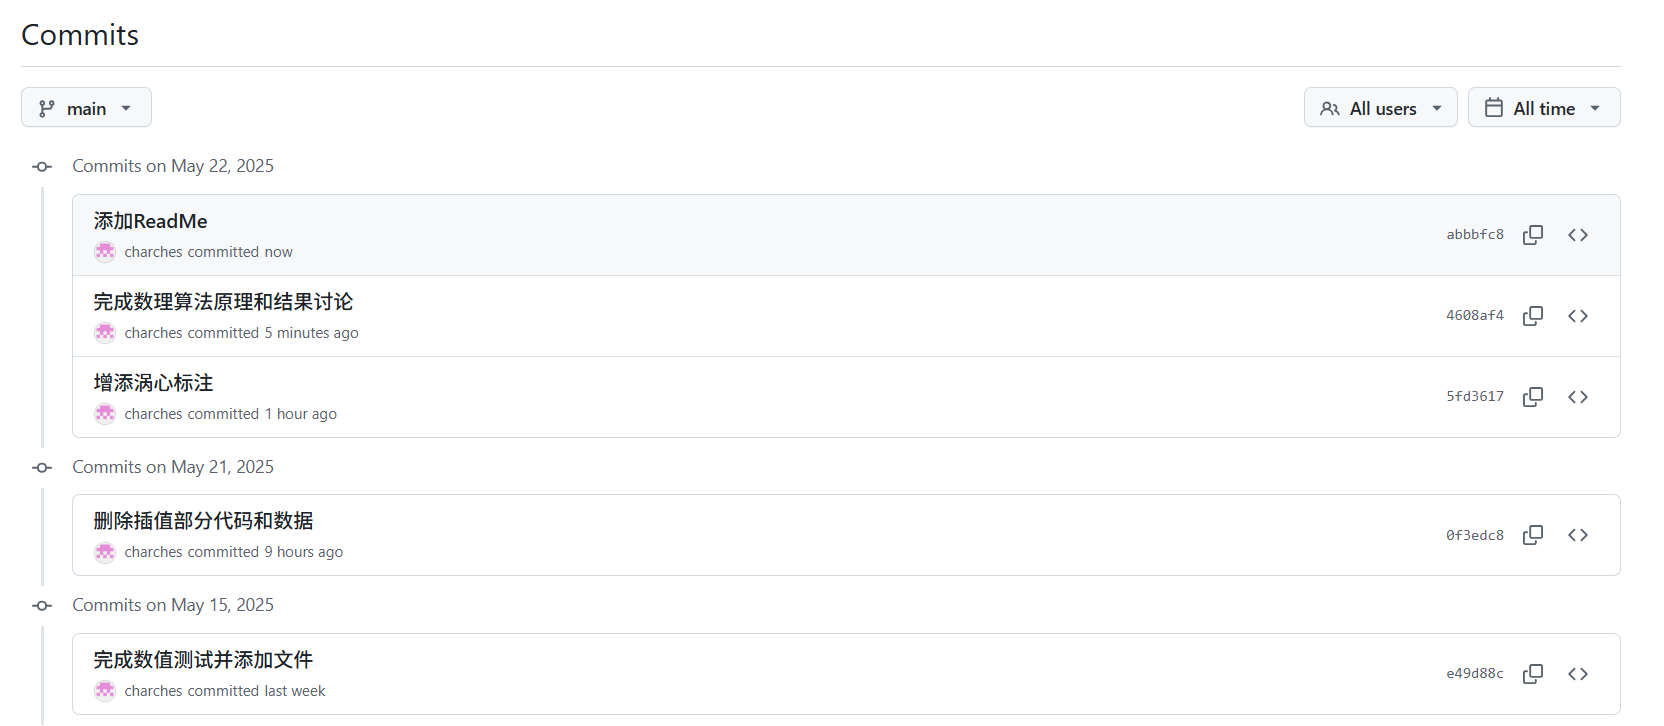
\includegraphics[width=0.8\textwidth]{./pictures/git_control.png}
\end{figure}
\end{document}